\subsection{Оценка влияния нелинейного элемента на свойства линейной системы}
Для исследования влияния НЭ нужно рассмотреть 2 системы: с НЭ и без него.
Структурная схема системы будет соответствовать СС на рис.\ref{fig:sim_PD} с наличием НЭ и и без него.
Из результатов предыдущего моделирования выберем коэффиценты $k_1=44.4444,k_2=165$. 
 Графики изменения выходной переменной $X$ для системы с НЭ и без него на рис.\ref{fig:NE_influence_sys} 
при подаче на вход ЕСФ
\begin{figure}[!h]\centering
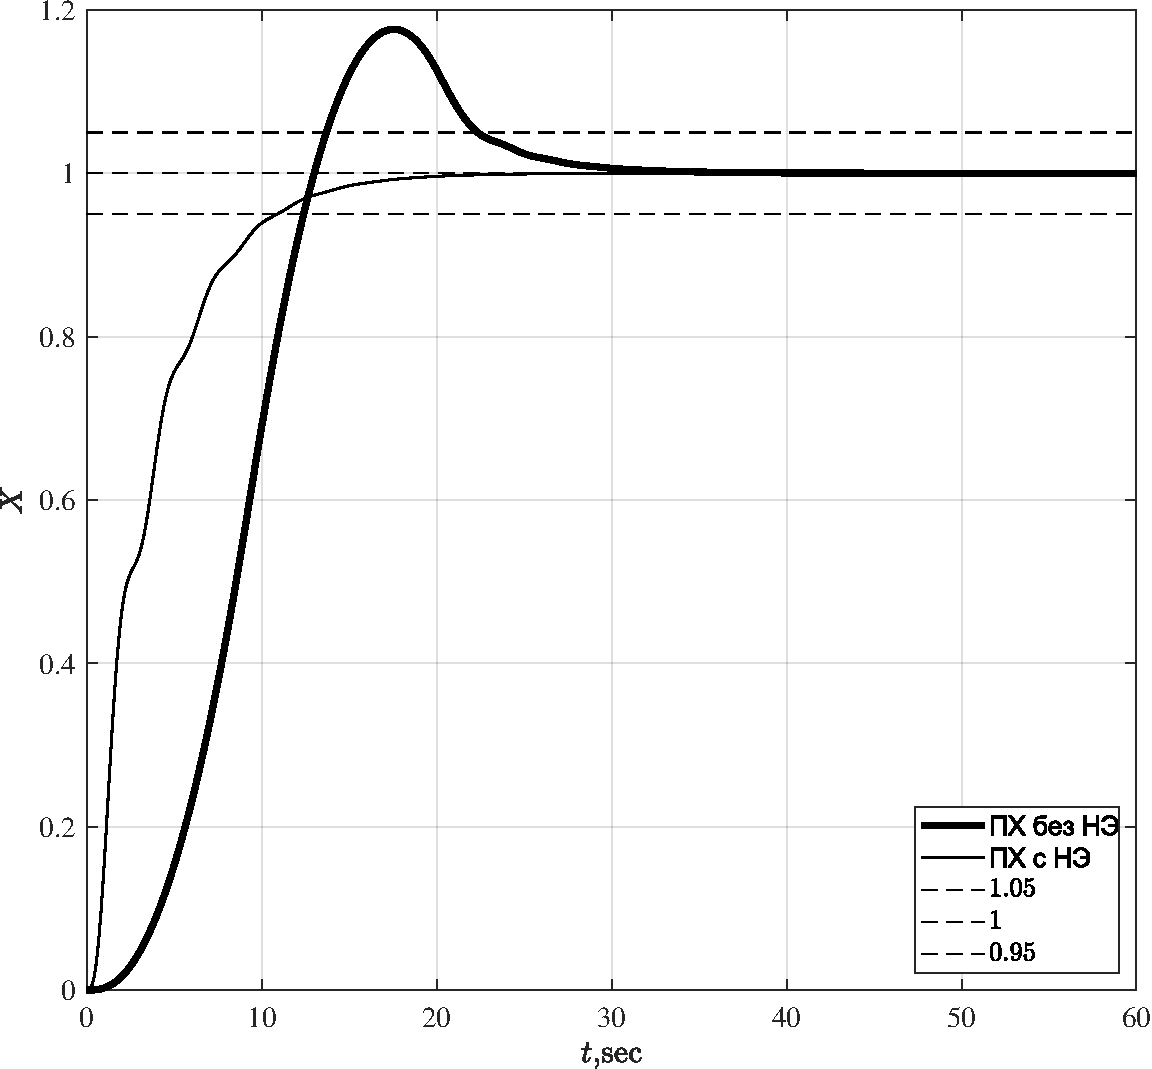
\includegraphics[width=1.0\linewidth]{images/NE_influence_sys}
\caption{ Графики изменения выходной переменной $X$}\label{fig:NE_influence_sys}
\end{figure}

